\documentclass[letterpaper, 10 pt, conference]{ieeeconf}

\IEEEoverridecommandlockouts
\overrideIEEEmargins

\usepackage{graphicx}
\usepackage[caption=off]{subfig}

\usepackage[tbtags]{amsmath}
\usepackage{amsfonts}

\usepackage{url}

\renewcommand{\vec}[1]{\boldsymbol{#1}}
\newcommand*{\R}[1]{\mathbb{R}^{#1}}

\def\figurename{Fig.}

\begin{document}

	\title{\LARGE \bf Task-Level Teleoperated Manipulation \\ for the HRP-2 Kai Humanoid Robot}

	\author{Rafael Cisneros, Takeshi Sakaguchi, Shuuji Kajita, \\
					Shin'ichiro Nakaoka, Mitsuharu Morisawa, Kenji Kaneko, Fumio Kanehiro
	\thanks{R. Cisneros, T. Sakaguchi, S. Kajita, S. Nakaoka, M. Morisawa, K. Kaneko and F. Kanehiro
					are with the Humanoid Research Group of the National Institute of Advanced Industrial Science
					and Technology (AIST), 305-8568 Tsukuba, Japan. {\tt\small rafael.cisneros@aist.go.jp}}}
  
	\maketitle

	\thispagestyle{empty}
	\pagestyle{empty}

	\begin{abstract}
		This paper presents the strategy used by our team, AIST-NEDO, at the DARPA Robotics Challenge (DRC) to deal
		with the designated manipulation tasks by means of a task-level teleoperation of the HRP-2 Kai humanoid robot,
		considering a disaster-hit scenario that is inherently non-structured and a limited communication between the
		user and the robot.
		The strategy, based on the information provided by a laser rangefinder (LRF) and a set of cameras installed
		at the head and at both hands, consisted in the alignment of 3D models representing the desired manipulation
		targets with a measured point cloud, in order to provide a reference frame to describe the manipulation motion
		required for each task.
		Each motion was carefully planned in advance by assuming minimum information of the object representing the
		manipulation target.
		In order to exemplify the before mentioned approach, three representative tasks of the DARPA Robotics Challenge
		are described, as well as the corresponding results obtained during the competition.
	\end{abstract}

	\section{Introduction and Motivation}
	\label{sec:introduction}

	Disaster response is attracting attention from the robotics research community, and even more since the
	Fukushima Daiichi nuclear power plant accident that followed the 2011 Great East Japan earthquake and tsunami.
	As a concrete materialization of this increasing interest, a challenge is proposed by the American Defense
	Advanced Research Projects Agency (DARPA) to use robots in disaster-hit facilities that were made too hazardous
	for direct human operator intervention.
	It is worth noticing that the challenge does not impose any constraint on the design of the robot, but since the
	environment (industrial ladders, doors, valves, cars) as well as the tools (levers, drills, hammers) were meant
	to comply with the human morphology, it is a natural option to develop the necessary means to make the humanoid
	robots capable of performing inspection and disaster recovering actions inside a non-structured environment
	\cite{Bouyarmane}.
	
	This environment can be considered to be ``kind of'' known in the sense that we know which actions
	(the type of tasks)	are required in advance and that we have a rough idea of its spatial distribution,
	maybe altered due to the disaster itself.
	However, it is assumed that there is no precise model of this environment, and that there are previously unknown
	obstacles, randomly placed on it.
	
	Despite of these conditions, the robot must be able to travel through the environment to achieve a proper stance
	with respect to the object(s) representing the target of the task, such that they be inside of the dextrous
	workspace of the hands of the robot.
	
	It is also mandatory to consider that within a desaster-hit facility it is not possible to rely on a stable,
	wide bandwidth communication system.
	
	% Still working on this
	This has to be done by means of a task-level teleoperation
	
	\section{Related Work}
	\label{sec:related_work}
	
	From some years ago, there has been plenty of research on fully autonomous robots capable of performing
	tasks in structured environments (kitchens, offices, etc.), as the one presented by Blodow et al~\cite{Blodow}
	or Beetz et al~\cite{Beetz}.
	For that purpose many different control architectures have been proposed, some of them are described by
	Medeiros~\cite{Medeiros}.
	For non-structured environments there is one basic paradigm called \emph{supervised autonomy},
	proposed first by Cheng and Zelinsky~\cite{Cheng}, which has become the current state of art for
	the DARPA Robotics Challenge (DRC) since the Trials and also for the Finals.
	During these competitions, each team relied on an Graphic User Interface (GUI) showing the a 3D model of the
	robot and the environment, in such a way that the operator(s) could control the robot beyond the joint-level,
	by specifying task-level commands that were robot-centric and/or object centric, as described by the teams
	Tartan Rescue~\cite{Dellin}, MIT~\cite{Fallon}, RoboSimian~\cite{Hebert} and ViGIR~\cite{Romay}.
	In this paper, we describe our implementation of this approach.	
	
	\section{HRP-2 Kai humanoid robot}
	\label{sec:hrp2kai}
	
	\begin{figure}[t]
		\begin{center}
			\subfloat[Actual robot.]{\label{fig:HRP2Kai-robot}
				\includegraphics[height = 6cm]{img/HRP2Kai-robot}}
			\hspace{1cm}
			\subfloat[Kinematic structure.]{\label{fig:HRP2Kai-structure}
				\includegraphics[height = 6cm]{img/HRP2Kai-structure}}
		\end{center}
		\caption{HRP-2 Kai humanoid robot.}
		\label{fig:HRP2Kai}
	\end{figure}
	
	\section{Teleoperated Manipulation Method}
	\label{sec:teleop_manip_method}
	
	Let us consider a humanoid robot equipped with a Laser Range Finder (LRF) placed at the head,
	as well as three cameras: at the head and at each hand.
	The LRF provides a point cloud of the environment, probably contaminated with noise due to the enviromental
	conditions of the disaster scenario; that is, even after a proper calibration it is not possible to consider
	that the 3D data precisely represents points belonging to objects in the environment, but within a certain
	amount of tolerance.
	On the other hand, the frame rate of the cameras, as well as the resolution, are intentionally set low
	foreseeing the effects of the degraded communication.
	
	This information of the environment, together with the sensorial information providing the current state of
	the robot, are the only information available to the operator, which has to supervise the robot while performing
	the tasks by establishing	high level goals, assisting with perception and changing parameters during the task.
	For this purpose, and under the circumstances stated above, we came up with a teleoperated manipulation method
	based on ``markers'' which assume minimum knowledge of the environment.
	This one is explained on the following.
	
	\subsection{Approaching to the target}
	
		The robot must achieve a proper stance with respect to the object(s) representing the target of the task,
		such that they be inside of the dextrous workspace of the hands of the robot.
		To do that the robot must perform a first measurement of the environment in order to check, together with the
		head camera, if the manipulation target is represented by some set of points of the resulting point cloud.
		In such a case, a preliminar alignment of a 3D object representing this manipulation target
		(the \emph{manipulation marker}) is first performed.
		
		By using the Graphical User Interface (GUI) provided by Choreonoid~\cite{Nakaoka_Choreonoid}, the Manipulation
		Marker is represented as the corresponding 3D model together with a set of arrows and rings which allow the
		operator to translate and rotate it with respect to its local reference frame,
		as depicted in \figurename~\ref{fig:ManipulationMarker}.
		
		\begin{figure}[b]
			\centering
			\includegraphics[height = 5.5cm]{img/ManipulationMarker}
			\caption{Manipulation Marker of a valve.}
			\label{fig:ManipulationMarker}
		\end{figure}

		Doing this alignment manually can be tedious, besides the fact that it may require a lot of time.
		To speed it up, it is possible to use a built in function included in the Point Cloud Library (PCL) that
		automatically alignes the marker with the best fit set of points, by providing maximum displacements,
		the number of iterations and some allowable error.
		However, ordinarily the robot will not be close enough to the object(s) for them to be measured with enough
		density of points, in such a way that the automatic alignment be prone to fail.
		One way to overcome this problem is to select one point of the point cloud belonging to the object and set
		this as the origin of the local reference frame of the Manipulation Marker, then the automatic alignment
		will lead to an alignment that may or may not require further small manual adjustments.
		
		One way to improve the initial alignment of the Manipulation Marker is to use beforehand information of the
		possible attitude of the object with respect to the nearest wall.
		For example, if the manipulation target is a box attached to the wall, its front face will probably be
		parallel to it.
		Knowing this, it is just the matter to identify the plane of the wall (and maybe the floor),
		get its mathematical representation and use it to define an initial attitude of the Manipulation Marker,
		requiring little automatic or manual adjustments.
		
		Once this is done, it is possible to define a proper stance of the robot (decided beforehand) with respect
		to the local reference frame of the Manipulation Marker.
		Then, by taking into account the height field of the floor (obtained from the point cloud) and avoiding the
		obstacles of the environment (walls and/or other objects), a proper footstep planning is performed in order
		for the humanoid robot to arrive to the desired stance~\cite{Morisawa}~\cite{Perrin}.
		
	\subsection{Grasping the target}
		
		Once humanoid the robot arrives to the desired stance, it has to perform another measurement.
		First, because of the positioning errors accumulated during its locomotion, and second,
		in order to obtain a more dense point cloud inteded for refining the alignment of the Manipulation Marker.
		
		Having done this refinement, it is possible to describe the attitude of the hands of the robot with respect
		to the local reference frame of the Manipulation Marker in order to approach to the manipulation target and
		grasp it, push it or pull it as required.
		Once decided, the whole-body Inverse Kinematics (IK) solution must be found, taking into account the redundancy
		of the robot to avoid collisions with the environment (represented with the point cloud)~\cite{Kanoun}.
		
		This relative attitude of the hands needs to be previously decided, such that the task be effectively carried
		out by means of smooth motions; that is, avoiding singular configurations and critical postures that may
		compromise the stability of the robot.
		However, these ones can be modified during the execution of the task if necessary, by means of a Hand Marker,
		a 3D representation of the hand and a set of arrows and rings which allow the operator to translate and rotate it
		with respect to its local reference frame, calculating at the same time the resulting configuration of the
		humanoid robot.
		See \figurename~\ref{fig:HandMarker}.
		
		\begin{figure}[b]
			\centering
			\includegraphics[height = 5.5cm]{img/HandMarker}
			\caption{Left Hand Marker.}
			\label{fig:HandMarker}
		\end{figure}
		
	\subsection{Dealing with uncertainties}
		\label{sub:uncertainties}
		
		Grasping the target with the desired relative attitude can be critical for some manipulation tasks,
		specifically if the target size is small when compared to the hand.
		However, it is worth to consider that the point cloud has an intrinsec noise, mainly caused as a result of the
		sunlight which complicates measurements.
		Then, it is not advisable to rely completely on the point cloud to plan the grasping motion,
		as the shown points may not represent actual points on the objects.
		
		One way to overcome this problem is to place the robot's hand within the view field of the LRF,
		and add some offset to the point cloud in order to match the corresponding points with the hand,
		whose attitude is known.
		This strategy practically improves the representation of the target objects by the point cloud but
		the precision may not be high enough.
		However, it can be used to approach to the manipulation targets (within some centimeters) before grasping them,
		with enough confidence that the hand is not going to collide unintentionally with the environment.
		
		Having done this, it is possible to use an approaching strategy in which the hand intentionally collides with
		the target by means of a slow motion, in order to use the force sensor installed in the hand to stop the hand
		when it senses a force greater than some established offset.
		Then, the real position of some plane of the target can be known relative to the hand, whose attitude can be
		computed by using forward kinematics and the actual joint values.
		The grasping point on the target can then be reached by moving the hand a very small distance with respect
		to its local reference frame.
		
	\subsection{Manipulating the target}
		
		Once the target is grasped, the relative attitude between the Manipulation Marker and the Hand Marker(s) can be
		set to be constant.
		Then, it is possible to manipulate the target by translating / rotating the Manipulation Marker, such that the
		required configuration of the humanoid robot be automatically calculated by means of solving the corresponding
		whole-body IK problem.
		In this way, a broad range of manipulation tasks can be accomplished by following this scheme, as illustrated
		by some examples which are described as follows.
		
	\section{Pulling and inserting a plug}
	\label{sec:plug}
	
	\subsection{Outline of the plug task}
	
		One of the surprise tasks at the DRC consisted of pulling out a plug
		from one socket and putting it back into another socket, in a set-up like the one shown in
		\figurename~\ref{fig:Sockets-Plug}.
		The separation between both sockets was not known in advance, neither the height at which
		they were placed.
		Only the shape of the plug was known in advance.
		
		\begin{figure}[t]
			\centering
			\includegraphics[height = 3.5cm]{img/Sockets-Plug}
			\caption{Plug Task.}
			\label{fig:Sockets-Plug}
		\end{figure}
		
		To carry out this task, we can consider its execution as divided into the following phases:
		%
		\begin{enumerate}
			\item Detection the socket and plug.
			\item Grasping the plug.
			\item Pulling and adjusting the plug.
			\item Inserting the plug.
		\end{enumerate}
	
	\subsection{Detection of the socket and plug}
		
		In order to perform this task it is first necessary to identify the plug and the socket where
		it is originally inserted, by placing the corresponding Manipulation Marker within the point cloud.
		The reason to identify both objects instead of just the plug is because almost half of it
		is not visible, as it is inside of the socket.
		As a consequence, the matching precision attained by aligning just the plug is lower than the one
		attained by aligning both objects.
		
		To do that we first detect all the planes in the scene, assuming that one of them will correspond
		to the wall where the sockets are installed.
		Then, given that the front face of the sockets is parallel to this wall, it is possible
		to calculate their orientation with respect to the robot.
		Having done this, one point belonging to the plug can be manually selected in order to compute
		an approximate initial position for the Manipulation Marker representing the socket and the plug.
		
		This initial position can be later refined, after the robot has arrived to the desired stance and
		after the point cloud has been adjusted by using one hand of the robot as a reference
		(given that its attitude can be calculated from the internal sensors), as shown in
		\figurename~\ref{fig:SocketPlugMarker}.
		This is because the measured point cloud has some intrinsic noise, mainly caused as a result of
		the sunlight.
		
		\begin{figure}[b]
			\centering
			\includegraphics[height = 4.5cm]{img/SocketPlugMarker}
			\caption{Detection of the socket and the plug.}
			\label{fig:SocketPlugMarker}
		\end{figure}
		
	\subsection{Grasping the plug}
		
		Having detected an approximate attitude for the socket, the robot first approaches the plug
		with one hand while aligning the camera installed at the other hand with the axis of the plug.
		By doing this it is possible for the operator to make slight adjustments of the grasping hand
		by using the visual information provided by the hand camera.
		\figurename~\ref{fig:PreCloseHand} shows this configuration for the situation in which the plug
		is initially inserted into the left socket.
		Then, the robot uses its right hand to grasp the plug and the left hand for the camera.
		Were the plug initially inserted into the other socket, then the role for both hands would be
		reversed.
		
		\begin{figure}[t]
			\centering
			\includegraphics[height = 4.5cm]{img/PreCloseHand}
			\caption{Configuration of the robot before grasping the plug.}
			\label{fig:PreCloseHand}
		\end{figure}
		
		The size of the visible part of the plug is not that big compared to the hand of the robot,
		and because of that the allowable tolerance for grasping the plug is small.
		Then, it is required to grasp it at the point in which the hand also touches the socket.
		This can be done by translating the hand along the axis of the plug until sensing 30 N of force
		(enough for considering that it hits to the socket).
		This strategy is effective (when adjusted properly) as the grasp can be done every time at the
		desired point with enough precision even in the presence of uncertainties, as shown in the dynamical
		simulation depicted	in \figurename~\ref{fig:GraspPlug}.
		
		\begin{figure}[b]
			\centering
			\includegraphics[height = 4.5cm]{img/GraspPlug}
			\caption{The plug being effectively grasped.}
			\label{fig:GraspPlug}
		\end{figure}
		
	\subsection{Pulling and adjusting the plug}
		
		After grasping the plug, the robot has to pull it.
		Due to the waist motion occurring during the stabilization of the robot, the pulling motion may not
		be performed exactly along the axis of the plug, and this one may hit the inner walls of the socket
		while being pulled, modifying the planned relative attitude between the plug and the grasping hand.
		
		For this reason, before inserting the plug into the other socket, the robot first brings the plug
		in front of its chest, takes an updated point cloud, and uses the camera placed at the head and
		at the other hand to look at the plug from two perpendicular directions, as seen in
		\figurename~\ref{fig:WatchPlug}.
		By using the point cloud, together with the visual information of both cameras, it is possible to
		fix the actual attitude of the Manipulation Marker representing the plug to match the attitude of
		the real one with respect to the hand.
		
		\begin{figure}[t]
			\centering
			\includegraphics[height = 4.5cm]{img/WatchPlug}
			\caption{After pulling the plug its attitude is adjusted.}
			\label{fig:WatchPlug}
		\end{figure}
		
	\subsection{Inserting the plug}
		
		Once this relative attitude is known it is possible to align the plug with the destination socket,
		whose position can also be approximated by adjusting the corresponding marker within the point cloud.
		However, it is still worth to consider that this position may not be accurate enough,
		making it unfeasible to attempt an immediate insertion.
		Instead, the camera at the other hand can be used once again together with the camera at the head to
		look at the plug from two different points of view (as seen in \figurename~\ref{fig:InsertPlug}),
		in such a way that the operator can use this visual	information to slightly adjust the position of the
		plug before inserting it.
		
		\begin{figure}[b]
			\centering
			\includegraphics[height = 4.5cm]{img/InsertPlug}
			\caption{The plug is inserted by using visual feedback.}
			\label{fig:InsertPlug}
		\end{figure}
		
		Then, once the task is completed, the grasping hand opens and an updated point cloud is taken again,
		in order to plan the returning motion without hitting the cable of the plug.
		
	\subsection{Result at the DRC Finals}
		
		During the second day of the DRC Finals 2015 (June 6), HRP-2Kai was able to carry out
		the plug task within 16 minutes and 34 seconds, mainly because we were supervising every motion of the
		robot in order to prevent unexpected collisions, and also due to the blackouts that prevented us to make
		a faster identification of the plug in the point cloud.
		Even without knowing the disposition of the sockets within the field, HRP-2Kai was able to identify the
		plug, approach to it, grasp it, pull it and insert it into the other socket.
		Then, before returning to its home position, the hand of the robot grazed the plug and it fell down.
		However, the point corresponding to the task was granted, as the plug was inserted into the socket
		when the robot opened its hand.
		Some snapshots taken during the task at the DRC Finals are shown in \figurename~\ref{fig:plug-drc},
		together with the description of the current process in accordance with the explanation given before.
		
		\begin{figure}[t]
			\centering
			\subfloat[Identify plug in socket]
				{\label{fig:Plug_30_24_60} \includegraphics[height = 2cm]{img/Plug_30_24_60}}
			\subfloat[Adjust point cloud offset]
				{\label{fig:Plug_32_24_23} \includegraphics[height = 2cm]{img/Plug_32_24_23}}
			\\
			%
			\subfloat[Prepare for pre-grasping]
				{\label{fig:Plug_34_33_87} \includegraphics[height = 2cm]{img/Plug_34_33_87}}
			\subfloat[Align hand to grasp]
				{\label{fig:Plug_37_23_37} \includegraphics[height = 2cm]{img/Plug_37_23_37}}
			\\
			%
			\subfloat[Pull out the plug]
				{\label{fig:Plug_38_13_00} \includegraphics[height = 2cm]{img/Plug_38_13_00}}
			\subfloat[Identify plug in hand]
				{\label{fig:Plug_39_03_07} \includegraphics[height = 2cm]{img/Plug_39_03_07}}
			\\
			%
			\subfloat[Prepare for pre-insertion]
				{\label{fig:Plug_43_42_13} \includegraphics[height = 2cm]{img/Plug_43_42_13}}
			\subfloat[Plug is inserted]
				{\label{fig:Plug_44_51_93} \includegraphics[height = 2cm]{img/Plug_44_51_93}}
			%
			\caption{Plug task at DRC Finals on June 6~\cite{DARPA}}
			\label{fig:plug-drc}
		\end{figure}
		
		Table~\ref{tab:teams} summarizes the performance obtained by the teams that were able to
		accomplish the plug task.
		For comparison effects, the following information is presented:
		the place obtained by each team during the competition, the time spent during the execution
		of the plug Task, the effective time of the task (by considering only the time in which the
		robot is moving) and the number of adjustments performed during the insertion of the plug.
		
		\begin{table}[t]
			%
			\caption{Teams that completed the plug task.}
			\label{tab:teams}
			\centering
			%
			\begin{tabular}{cccccc}
				\hline
				Team 					& Place	& Task	& Effective & Insertion	\\
											& 			& time	& time			& adjust.		\\
				\hline
				KAIST					& 1			& 11:01	& 2:18			& 14				\\
				IHMC Robotics	& 2			& 6:31	& 2:32			& 8					\\
				Tartan Rescue	& 3			& 18:33	& 3:21			& 17				\\
				NIMBRO Rescue	& 4			& 8:16	& 2:29			& 16				\\
				WPI-CMU				& 7			& 5:07	& 1:42			& 7					\\
				AIST-NEDO			& 10		& 16:34	& 1:34			& 3					\\
				\hline
			\end{tabular}
			%
		\end{table}
		
	\section{Opening a box and pressing a button}
	\label{sub:button}

	\section{Door task}
	\label{sub:door}

\subsection{Outline}
%
The door task consists of the following four sequential steps.
%
\begin{description}
\item{Step1} Locate a door in the environment
\item{Step2} Walk to the front of the door and grasp the door knob
\item{Step3} Turn the knob and open the door
\item{Step4} Walk through the door
\end{description}
%

%In the DRC Finals, it was announced that the door will be 
%
%\begin{itemize}
%\item push open style,
%\item with lever type door knob, and
%\item without door closer.
%\end{itemize}

To realize a reliable door passing, we pre-determined
a robot pose grasping the door knob.
Let us call it as {\it door approaching pose} which specifies the
wrist point and the standing point with respect to the door lever
as illustrated in \figurename~\ref{fig:door_approaching_config}.

From Step1 to Step2, we control our robot to realize the door approaching pose.
The door knob operation (Step3) and the door passing through (Step4) always start
from this fixed configuration. This means we can use a programmed sequence or its minimum
modification at the door task.  

\begin{figure}[t]
  \centering
  \includegraphics[width = 6cm]{img/door_approaching_config}
  \caption{Door approaching pose}
  \label{fig:door_approaching_config}
\end{figure}
        
\subsection{Detection of the door lever}
%
For a door task, a robot must detect the door orientaion and the position 
of the door lever. We took two step manual operations to extract the required information
from the point cloud. % as illustrated in Fig.\ref{fig:door_manip_markers}.

First, an operator specifies an ``attention point'' on the point cloud which might correspond the 
left edge of the door panel (\figurename~\ref{fig:door_manip_markers}(a)). We can expect a flat plane 
on the right of the attention point, and we can calculate the orientation of the door plane by the least square method.
In \figurename~\ref{fig:door_manip_markers}(b) shows the automatically alligned ``door manipulation marker.''
The marker covers a part of the door panel and we can interactively manipulate it on the 
pointcloud GUI. By manually translating the marker, we can mask the flat portion of 
the point cloud and extract the door lever as shown in \figurename~\ref{fig:door_manip_markers}(c).
Since the door lever is relatively small with respect to the point cloud resolution,
it contains only 10 to 20 points which makes conventional model fitting very difficult.
Thanks to the robustness of the human perception, we can confidently assume the rotation center of the lever
 and the model allignment on the point cloud as \figurename~\ref{fig:door_manip_markers}(d).

\begin{figure}[t]
  \centering
  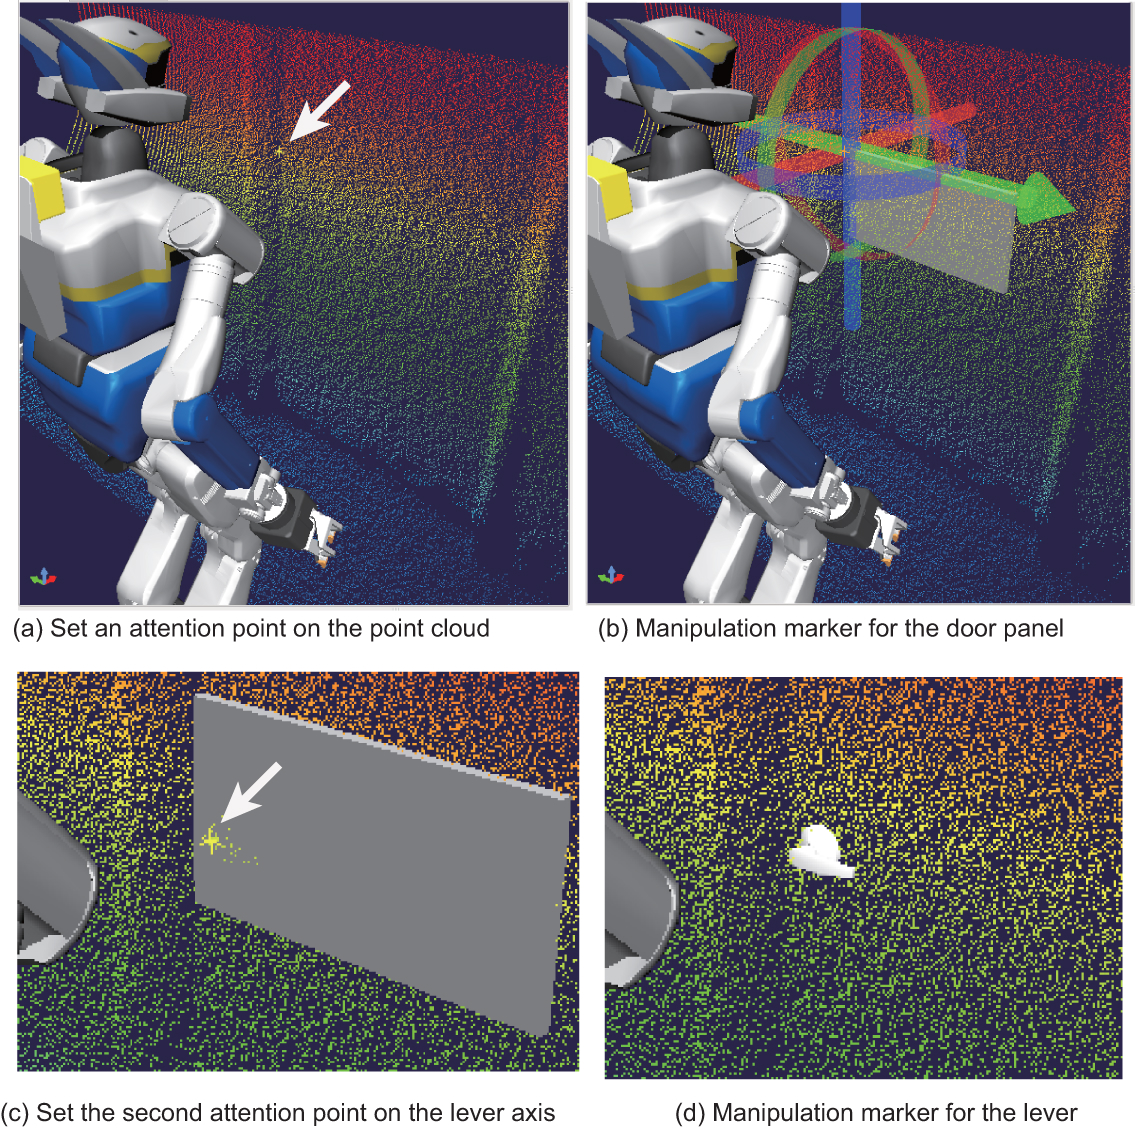
\includegraphics[width = 7.5cm]{img/door_manipulation_markers}
  \caption{Detection of the door lever in the control window}
  \label{fig:door_manip_markers}
\end{figure}
		

\subsection{Door lever grasp and manipulation}
%
By the method of previous subsection, we can expect 
our robot is standing in front of the door aligned to its surface normal with desired
distance. 
Nevertheless, due to the LRF measurement noise and its callibration error,
the hand position may not be acculate enough to grasp the lever. Such state in the dynamic simulation 
of Choreonoid is shown in \figurename~\ref{fig:door_lever_grasp}(a). 
The right window shows the simulated robot and the left 
window shows the view of the left hand camera. An operator can fix this manually by the GUI buttons of 
'Left','Right','Down', and 'Up' as seen in the left window bottom. In this case, an operator
can adjust the hand position by clicking 'Right' button several times.
Figure \ref{fig:door_lever_grasp}(b) shows the adjusted hand position to grasp the lever.
By hitting the button `OK', the robot move the left hand forward until it contacts the door surface (we specified a sleshold of 5N to detect the contact).  The hand is in contact with appropriate position to grasp the door lever in \figurename~\ref{fig:door_lever_grasp}(c).
   

\begin{figure}[t]
  \centering
  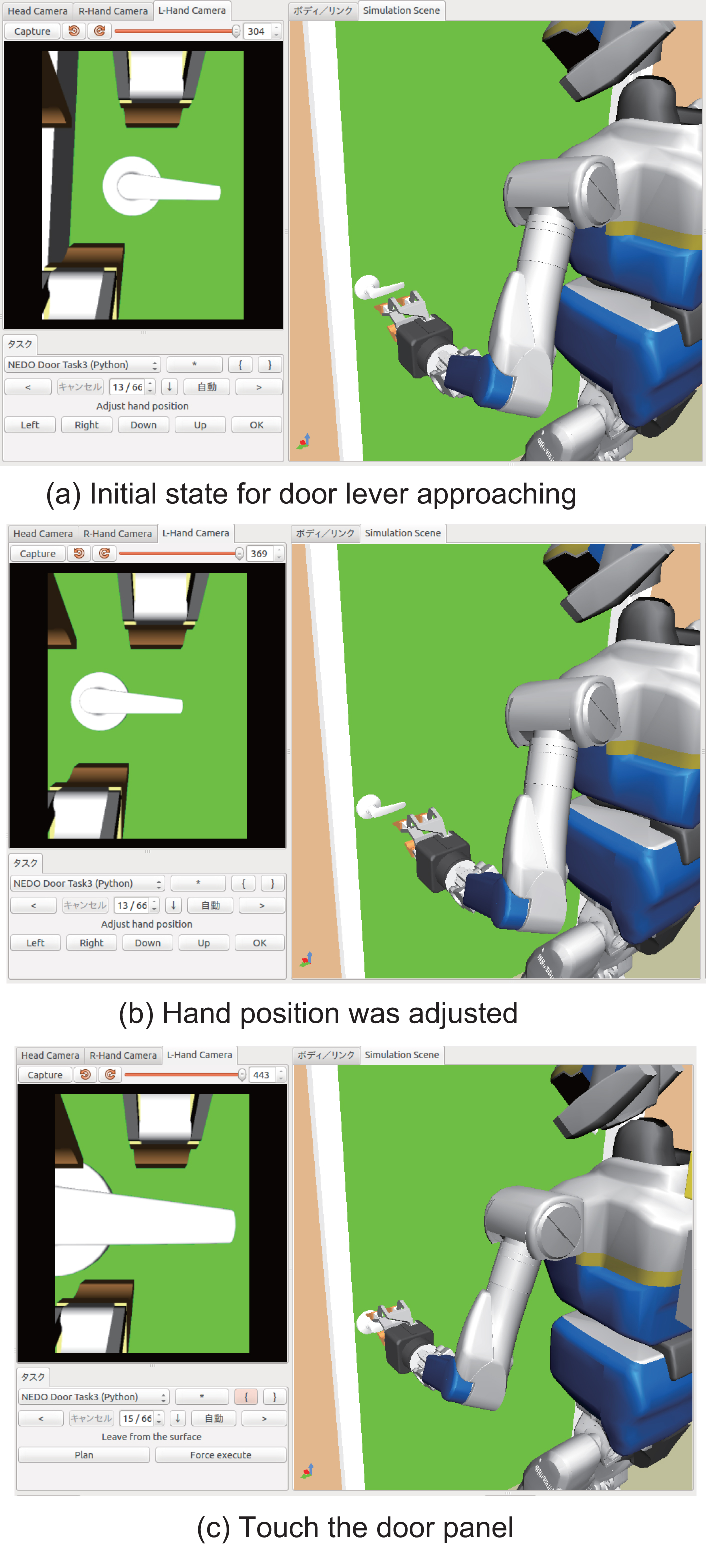
\includegraphics[width = 7.5cm]{img/approach_door_lever}
  \caption{Approach for door lever grasping}
  \label{fig:door_lever_grasp}
\end{figure}

%\begin{figure}[t]
%  \centering
%  \includegraphics[width = 7.5cm]{img/open_the_door.eps}
%  \caption{Door opening}
%  \label{fig:door_opening}
%\end{figure}

\subsection{Results at DRC Finals}
%
In the DRC Finals, the task stage floor has a slope of 2.6 degrees by 
our measurement, and the door was set perpendicular to the slope. 
By this setup, once the door was enough opend it quickly open by gravity
and remained opening state. This helped a lot our robot to pass the door.

On the other hand, we found that the door of each course has a different latch property
as shown in Table.\ref{tbl:door_latch}.

%
\begin{table}[htb]
\caption{Door latch properties at DRC finals} \label{tbl:door_latch}
\begin{tabular}{lclc}
\hline
Course & Lever angle to open & Date & Result  \\ 
\hline
Green & 30 deg & June 4 (rehasal) & Success  \\
Yellow & 70 deg & June 5 (day1) & Fail \\
Blue &  50 deg & June 6 (day2)  & Success \\
\hline
\end{tabular}
\end{table}

our robot had a trouble on turning the lever and releasing the latch.
		
	\section{Results}
	\label{sec:results}
	
	\begin{figure}[t]
		\centering
		\includegraphics[height = 5.5cm]{img/door-drc}
		\caption{Door Task at the DARPA Robotics Challenge~\cite{DARPA}.}
		\label{fig:door-drc}
	\end{figure}
	
	\begin{figure}[t]
		\centering
		\includegraphics[height = 5.5cm]{img/button-drc}
		\caption{Button Task at the rehersal of the DARPA Robotics Challenge~\cite{DARPA}.}
		\label{fig:button-drc}
	\end{figure}
	
	With respect to the plug task, during the DRC Finals we were able to complete the task
	and get the point	within 16 minutes and 34 seconds, mainly because we were supervising
	every motion of the robot in order to prevent any collision with the environment, and
	also due to blackouts.
	Some snapshots taken during the task at the DRC Finals are shown in
	\figurename~\ref{fig:plug-drc}, together with the description of the current process
	in accordance with the explanation given before.
	
	\begin{figure}[t]
		\centering
		\subfloat[Adjust manipulation marker]
			{\label{fig:Plug_30_24_60} \includegraphics[height = 2cm]{img/Plug_30_24_60}}
		\subfloat[Adjust point cloud offset]
			{\label{fig:Plug_32_24_23} \includegraphics[height = 2cm]{img/Plug_32_24_23}}
		\\
		%
		\subfloat[Adjust hand for pre-grasping]
			{\label{fig:Plug_34_33_87} \includegraphics[height = 2cm]{img/Plug_34_33_87}}
		\subfloat[Align hand to grasp]
			{\label{fig:Plug_37_23_37} \includegraphics[height = 2cm]{img/Plug_37_23_37}}
		\\
		%
		\subfloat[Pull out the plug]
			{\label{fig:Plug_38_13_00} \includegraphics[height = 2cm]{img/Plug_38_13_00}}
		\subfloat[Adjust manipulation marker]
			{\label{fig:Plug_39_03_07} \includegraphics[height = 2cm]{img/Plug_39_03_07}}
		\\
		%
		\subfloat[Adjust hand for pre-insertion]
			{\label{fig:Plug_43_42_13} \includegraphics[height = 2cm]{img/Plug_43_42_13}}
		\subfloat[Plug is inserted]
			{\label{fig:Plug_44_51_93} \includegraphics[height = 2cm]{img/Plug_44_51_93}}
		%
		\caption{Plug Task at the second day of the DARPA Robotics Challenge~\cite{DARPA}}
		\label{fig:plug-drc}
	\end{figure}
	
	\section{Conclusions}
	\label{sec:conclusions}
	
	The task-level teleoperation strategy presented in this paper was successfully applied
	to the HRP-2Kai humanoid robot, which was able to carry out all the manipulation tasks
	proposed for the DRC, even though there was no accurate model of the environment.
	Our principal restriction was the time limit, considering that most of the time spent
	during the task was the one required by the manual identification of the objects in the
	environment and by the verification of the robot motion by the operator.
	
	With respect to the plug task it is worth to notice that even though its execution
	lasted 16:34 minutes, the effective time was just 1:34 and the number of adjustments
	required to insert the plug was only 3.
	This was the result of assuring a stable grasp of the plug, as well as the use of markers
	to identify the plug and the sockets.
	
	As a future work we want to improve our recognition system, in order to speed up the execution
	of every task.
	
	\bibliographystyle{unsrt}
	\bibliography{ManipulationDARPA}
	
\end{document}